\documentclass[11pt]{article}
\usepackage[utf8]{inputenc}
\pagestyle{headings}
\usepackage[top=1in, bottom=1in]{geometry}
\usepackage{amsmath,amsfonts,amsthm,amssymb}
\usepackage[pdftex]{graphicx}
\usepackage{url}
\usepackage{subfig}
\usepackage{color}
\usepackage[pagebackref=true,breaklinks=true,letterpaper=true,colorlinks,bookmarks=false,citecolor=red,linkcolor=blue]{hyperref}

%% Command definitions
\def\subsectionautorefname{section}
\newcommand{\note}[1]{\textcolor{red}{\textbf{#1}}}
\definecolor{light-gray}{gray}{0.3}
\newcommand{\aside}[1]{\textcolor{light-gray}{\emph{#1}}}
\newcommand{\comment}[1]{}

\title{Attentional Object Detection: A Proposal}
\author{Sergey Karayev}
\date{updated: 22 April 2011}

\begin{document}
\maketitle

\begin{abstract}
This document tracks the development of ideas for efficient object detection using the idea of attention: a sequential process of looking for something somewhere.
We follow the Deformable Part Model approach to object detection and extend it in several ways, mostly focusing on the role of context, toward the goal of Anytime detection performance.
I expect a submission to NIPS'11 to be whittled down from the text and results here.
\end{abstract}

\tableofcontents
\newpage

\section{Introduction}

In recent years, the computer vision field has converged on a general method for object detection, and a standard evaluation of results.
Most current state-of-the-art object detection systems consist of three tasks: proposing regions of the image, evaluating a given region for presence of an object of a given category, and post-processing the results.
In the evaluation ground truth, each object is most commonly assumed to belong to one of a fixed set of classes; its location is approximated by placing a bounding box around pixels belonging to it.
Large datasets of such human annotations are used for evaluation of detection algorithms~\cite{pascal-voc-2010,imagenet_cvpr09}.

With few exceptions, current detection systems are not inherently multi-class.
Instead, separate detectors are trained per class, and they are deployed and evaluated independently.
The evaluation of multi-class performance, if at all given, consists of averaging the per-class metrics.
Some notable papers do make multi-class detection a priority, and accordingly evaluate in a multi-class setting, where false positives can be generated both by incorrect localization and incorrect labeling.
State-of-the-art detection systems also do not generally make efficiency a goal.

\begin{figure}[ht!]
\center{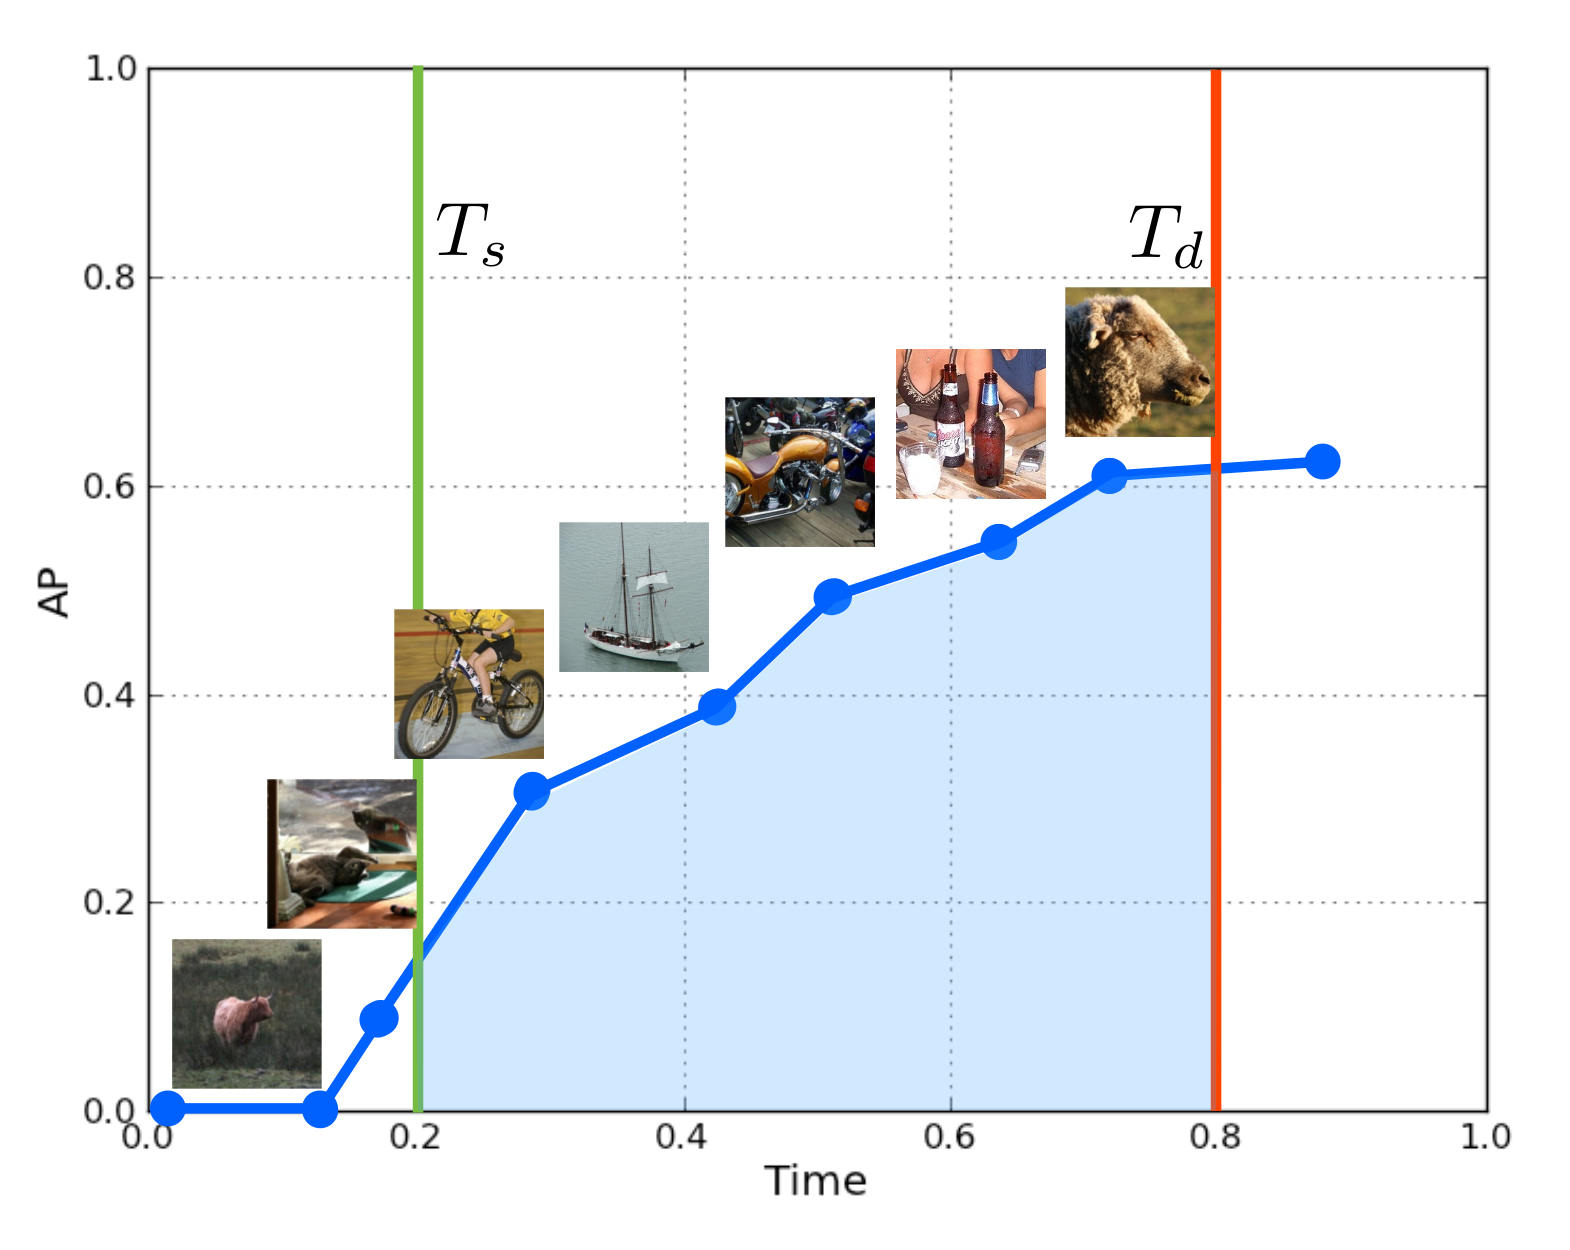
\includegraphics[width=0.56\linewidth]
    {figures/evaluation_thumbs.png}}
  \caption{We aim for \emph{Anytime} performance within the bounds of the curve. That is, the policy should give the best possible answer at any time from start time $T_s$ to deadline $T_d$.}
  \label{fig:evaluation}
\end{figure}

It is of course important to refrain from locking object recognition research into a single detector architecture with a focus only on increasing efficiency.
That said, there are applications for which performance truly is time-sensitive.
In robotics, a small finite amount of processing power per unit time is all that is available for robust object detection if the robot is to usefully interact with humans.
In large-scale detection system deployments, such as for image search, results need to be obtained quickly per image as the number of images to process is large and growing.
When processing large photo collection on end-user machines for immediate consumer navigation, the same is true.

In all these cases, an acceptable answer at a reasonable time may be more valuable than the best answer given too late.
Furthermore, the value of the answer depends largely on the target application.

A hypothetical recognition system for a vision-based advertising deployment presents a case study.
The system will have different accuracies for objects of different classes; detections will have different values based on confidence and class; and the queue of unprocessed images will vary in size.
The most rational detection strategy in such an environment should depend on all of these variables.

We argue that the key to tackling such problems of dynamic recognition resource allocation is to start asking a new question:
\emph{What is the best performance we can get on a budget?}
To answer it, we consider the evaluation metric of performance vs. time, presented in Figure~\ref{fig:evaluation} and discussed further in the text.

Our goal is a dynamic policy for selecting classifiers or detectors to achieve the highest recognition performance under this evaluation.

\section{Related Work}
The literature on object detection is vast.
Here we briefly summarize work relevant to our contribution.

An early success in efficient object detection used simple Haar features to build up a \emph{cascade} of classifiers, which then considered image regions in a sliding window regime~\cite{Viola2001}.
Plentiful later work improved the behavior of the cascade while maintaining the basic idea~\cite{Bourdev2005}. \note{more refs}
This detection method is fast, but the simple features and classifiers used have not led to the best performing detectors.

The best performance has recently come from detectors that use gradient-based features to represent either local patches or object-sized windows; if local patches are used, it appears important to include additional feature channels such as shape and color; if object-sized windows are used, finer-scale ``parts'' in object representation boost performance significantly.

%!TEX root=related_work.tex
\begin{figure}[h!]
  \caption{Most object detection approaches have three parts: region proposal, region evaluation, and post-processing of detections. The parts are in a sense sequential, which leads to the influence of cues like context being deferred to the post-processing stage, and to a dependency of early detections on the goodness of proposals. We present a system that considers region proposal and evaluation jointly, such that it is able to output the best detections early in the process.}
  \centering
    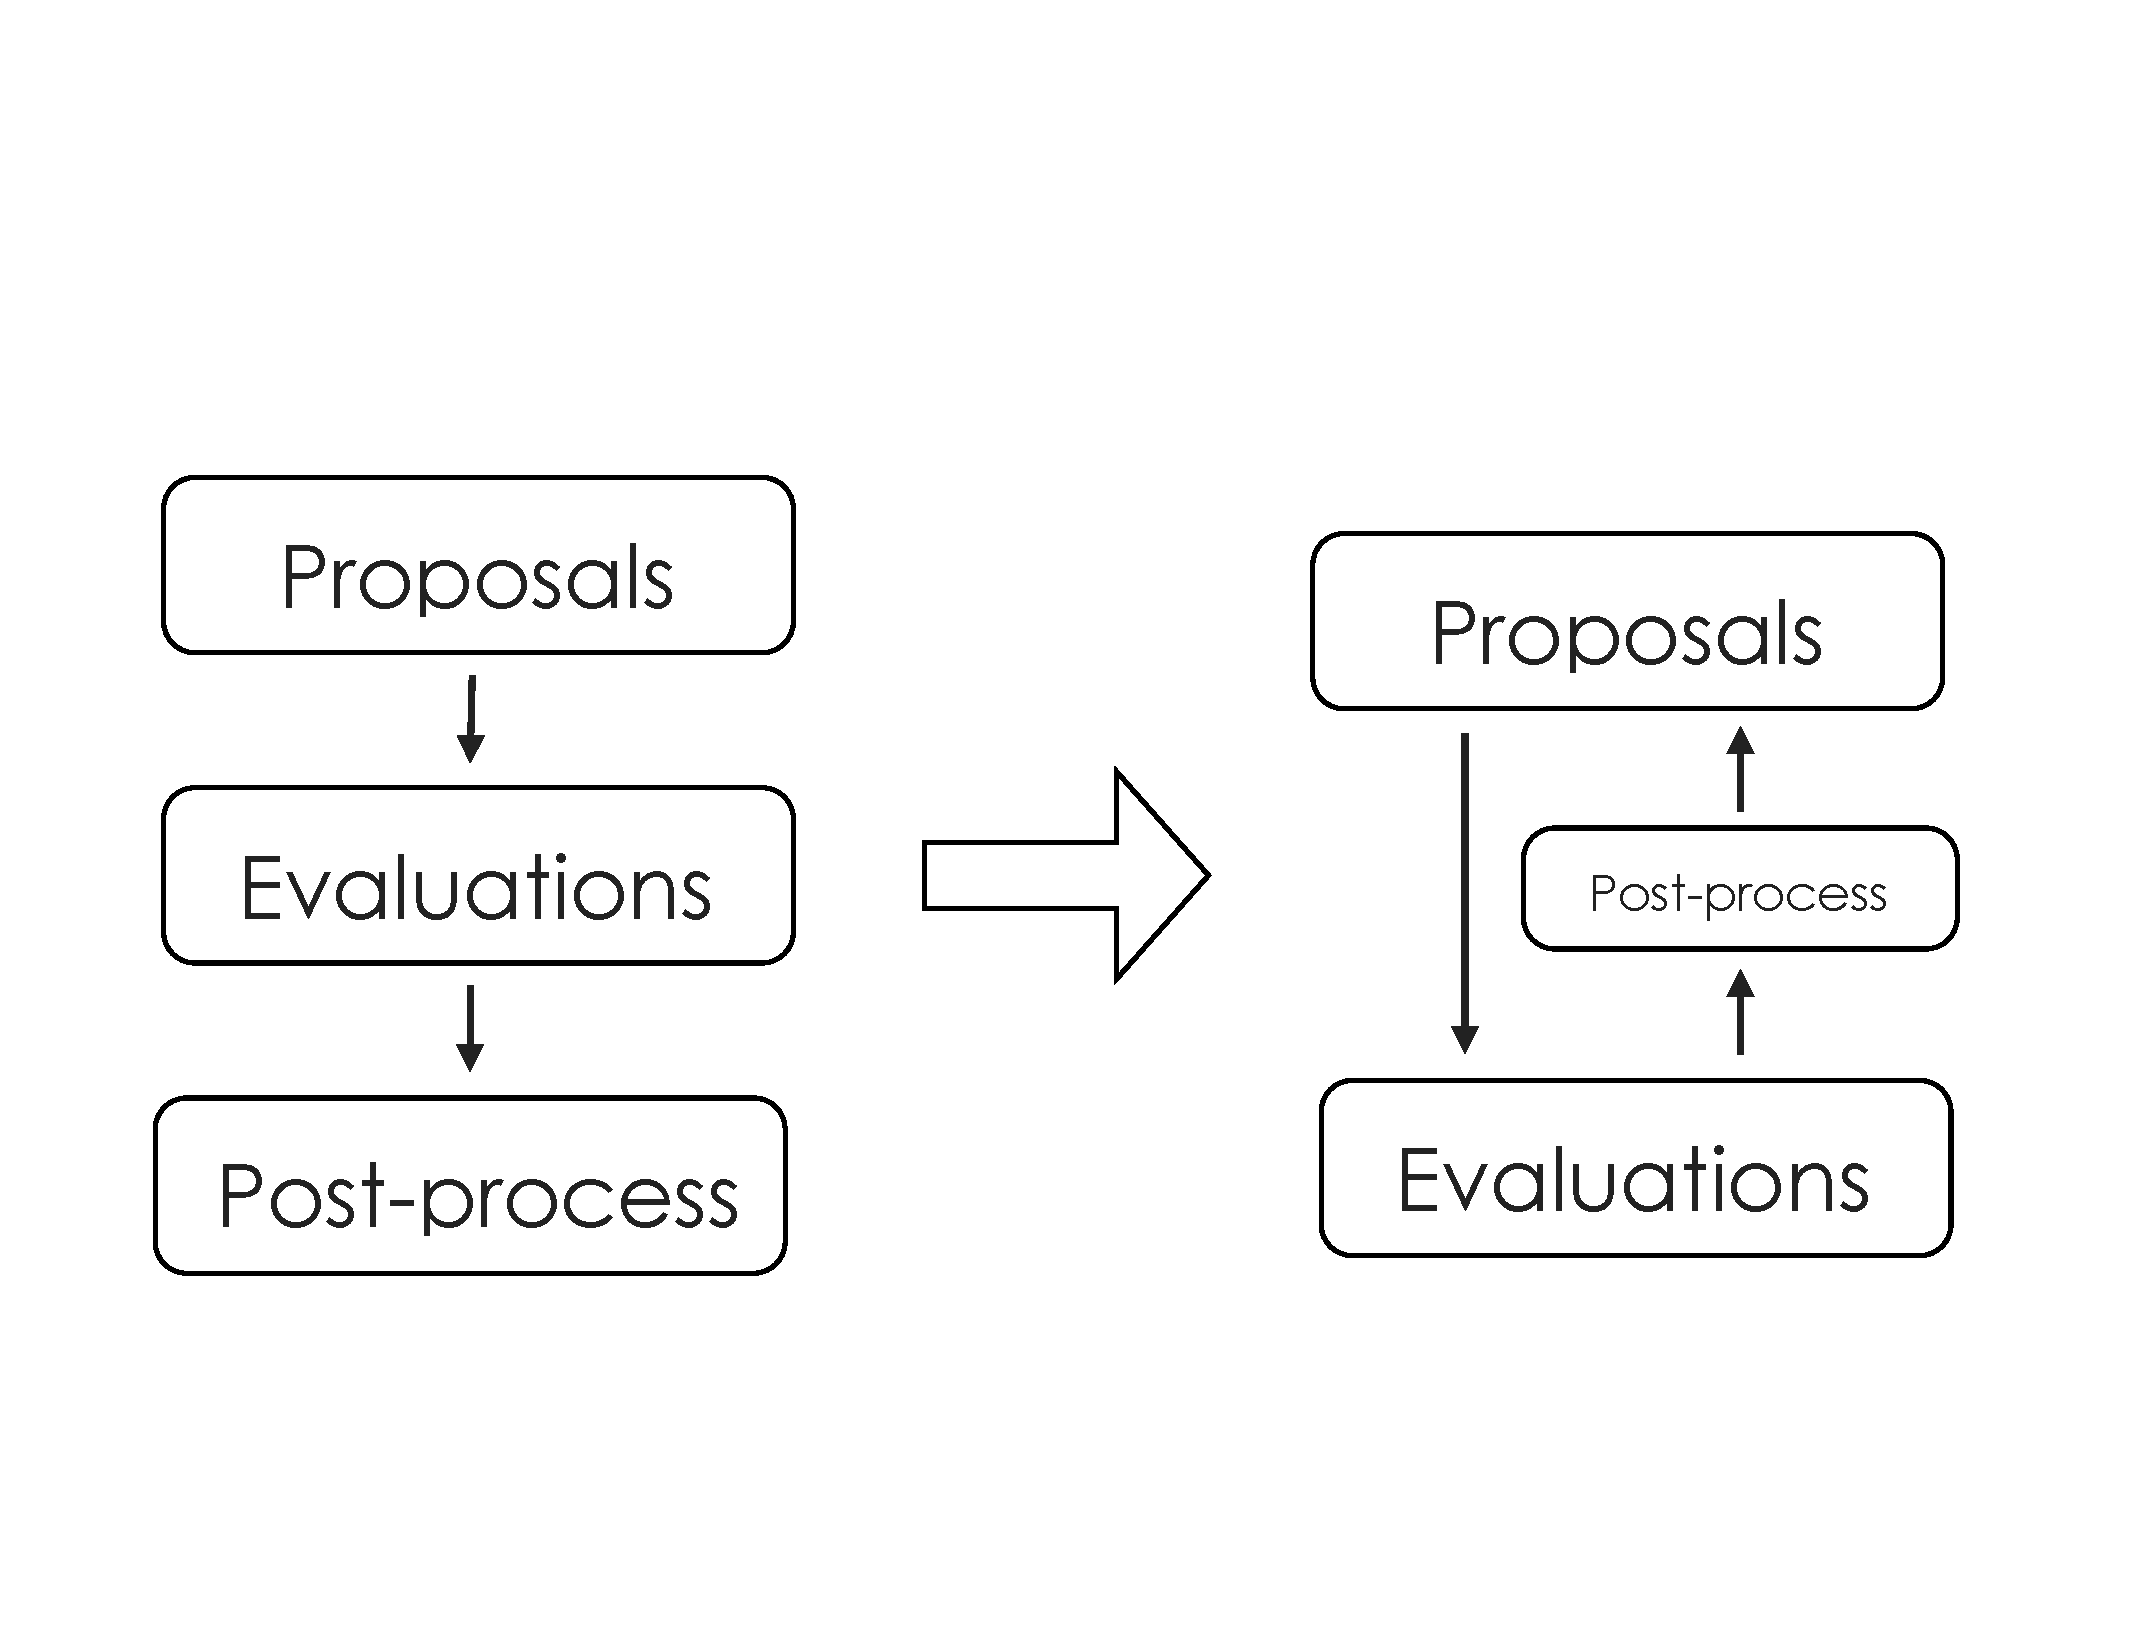
\includegraphics[width=0.9\textwidth]{../figures/architecture_concept.pdf}
  \label{fig:architecture_concept}
\end{figure}
Taking a grander view, most current detection systems can be conceptualized as having three parts, as visualized in~\autoref{fig:architecture_concept}.

The region proposal is usually done exhaustively over the image space, and doing so in an efficient order has not received much attention in the literature.
Using jump windows as region proposals is one common idea~\cite{Chum2007b,Vijayanarasimhan2011}.
For local features, a bounded search over the space of all possible windows works well (especially for single-object detection)~\cite{Lampert2008b}.
The method requires derivation of bounds, which have not yet been developed for HOG-based detectors, limiting the method's usefulness in state-of-the-art systems.
Similar ideas have been formulated in a decision theoretic way~\cite{Sznitman2010}.

Region proposal through segmentation is another common idea~\cite{Russakovsky2010}.
\note{more here.}

Another idea is to use a class-independent measure of ``objectness'' to reject much of the hypothesis space before running any class-specific detectors~\cite{Alexe2010,Endres2010}.
However, the latter approach has not been shown to be actually faster than exhaustive evaluation, either because the proposal step becomes too expensive~\cite{Endres2010}, or because the system was not coded efficiently~\cite{Alexe2010}.

In search of efficient detectors, the general ``cascade'' idea of breaking up the evaluation of an image region into thresholded steps has been applied to current state-of-the-art systems~\cite{Vedaldi2009, Felzenszwalb2010a}.
In the case of the Multiple-Kernel Detector~\cite{Vedaldi2009}, the cascade is necessary to keep detection of a single class to the order of a minute per image.
In the case of the Deformable Parts Model~\cite{Felzenszwalb2010a}, the cascade speeds up detection from several seconds to under a second per class, with little loss in accuracy.

Evaluation of regions involves feature computation, which is a time consuming step.
Efficient feature computation for HOG-based detectors has been explored in~\cite{Dollar2010}.
Another idea is coarse-to-fine model evaluation.
A recent work applies coarse-to-fine evaluation and adds a feedback arrow from post-processing to proposals, obtaining an order of magnitude speedup in the deformable part models framework while losing some accuracy~\cite{Pedersoli2011}.

Other systems that add feedback arrows to the conceptual diagram in~\autoref{fig:architecture_concept} are often inspired by biological vision and sequential decision process ideas~\cite{Butko2009,Vogel2008,Paletta2005}.
\note{more}

A close relative to this idea is inspired by the problem of tracking objects.
A recent paper draws an interesting feedback arrow from Evaluations to Proposals by using iterative sampling of a hypothesized mixture of Gaussians to find multiple objects in the image~\cite{Gualdi2010}.

Anytime performance in vision systems is a surprisingly little-explored idea.
A pioneering recent paper picks features with maximum value of information in a Hough-voting framework, and explicitly evaluates itself with regard to time \cite{Vijayanarasimhan2010}.

Multi-class detection has its own line of work, focusing largely on detection time sublinear in the number of classes through sharing features~\cite{Torralba2007,Fan2005,Razavi2011}.
An interesting reinforcement learning approach in a cascade framework is taken in~\cite{Isukapalli2006}.
\note{more}

A recent post-processing extension to detection systems uses structured prediction to incorporate multi-class context as a principled replacement for the common step of non-maximum suppression~\cite{Desai2009}.
This work aims to tie up a couple of loose threads of object detection: 1) joint multi-class detection, with the mutual exclusion and contextual effects it entails; 2) the hack of non-maximum suppression of single-class detections.

Context has a long history in vision.
One source of context is the scene or non-detector cues; for the PASCAL VOC, these are quantitatively considered in~\cite{Divvala2009}.
Another source is inter-object context, used for detection in a random field setting in~\cite{Torralba2004}.
\note{more}

Brief review of attentional modeling work~\cite{Itti2001a,Chikkerur2010,Judd2009}.
The concept of saliency has been used for object classification \cite{Kanan2010}.

\note{todo: active recognition~\cite{Denzler2002,Andreopoulos2009}.}

The two papers closest to our contribution are principled multi-class structured prediction~\cite{Desai2009} and the detection under bounded resources work~\cite{Vijayanarasimhan2010}.
We significantly extend the first work, which assumes that all classes have been evaluated at all regions, to the online case of picking regions and classes to evaluate.
We are guided by the same motivation of Anytime performance as the second work, but in a significantly more powerful detection regime.
Although we rely on the commonly used deformable parts model detector, our method can use any feature extraction and classification method.
\section{Evaluation} \label{sec:evaluation}

We use one-vs-all deformable part-model classifiers on a HOG featurization of the image \cite{Felzenszwalb2010a}, with associated linear classification of the detections.

\begin{figure}[h!]
\centering
\subfloat[Occurence of a class with another]{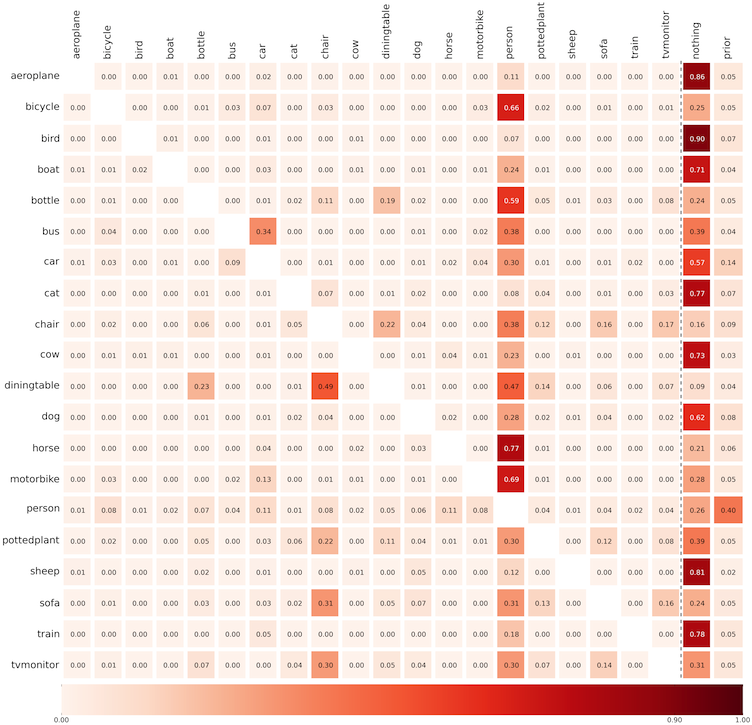
\includegraphics[]
    {../figures/full_pascal_trainval_stats/cooccur_trim.png}} \hfill
\subfloat[Occurence of a class with two others]{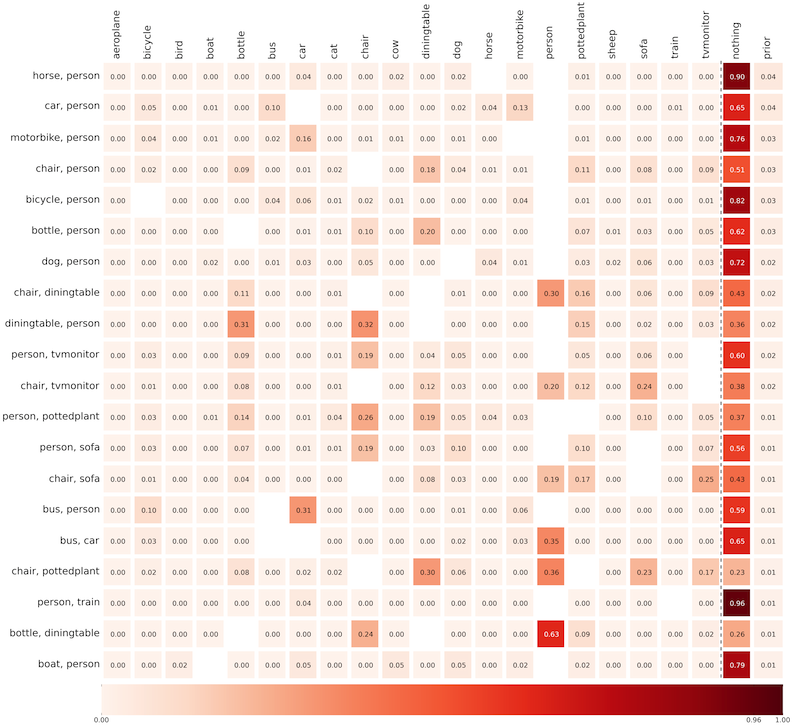
\includegraphics[]
    {../figures/full_pascal_trainval_stats/cooccur_second_order_trim.png}}
  \caption{
  Co-occurrence statistics on the training portion of the PASCAL VOC 2007 dataset.
  In the first plot, a (row,column) cell shows the probability that an image that contains an object of the row class also contains an object of the column class.
  Accordingly, in the second plot, the probability that an image containing objects of the two classes listed in the row also contains an object of the column class.
  }
  \label{fig:dataset_stats}
\end{figure}

To summarize \autoref{sec:}, we evaluate our system in the multi-class, multi-label detection regime.
We evaluate on a popular detection challenge task: the PASCAL VOC dataset \cite{pascal-voc-2010}.
As shown in \autoref{fig:dataset_stats}, the dataset exhibits a rather modest amount of class co-occurrence, which puts our model in a disadvantaged setting.
$60\%$ of the images in the training set have only one class; $30\%$ have two classes, $7\%$ have three classes, and almost none have more.

Using the 2007 version of the dataset, we train on the training and validation data and test on the test set.
We run our policies on all images in the test set, cutting off execution at $T_d$.

To evaluate performance at a given time, we gather all detections and the classification answers found to this point in all the recognition episodes.
As described before, we evaluate detection performance by averaging per-image performance in the multi-class regime.
We evaluate classification performance by pooling the ground truth across the dataset, in standard procedure.

We establish the baseline performance of our system by selecting actions randomly at each step.
The time setting for our evaluation is $T_s=0$, $T_d=20$ (in seconds).
As shown in Figure~\ref{fig:results_manual}, the random policy results in a roughly linear gain of performance vs. time.

To establish an upper bound on performance, we also plot the Oracle curve, obtained by re-ordering the actions with the hindsight of the results they produced.
Note that the curves turn downward in this setting: this is due to the different performance levels of the detectors: as the weaker detectors are inevitably run, they introduce more false positives and false negatives than true positives.

\begin{figure}[h!]
\centering
\subfloat[Detection]{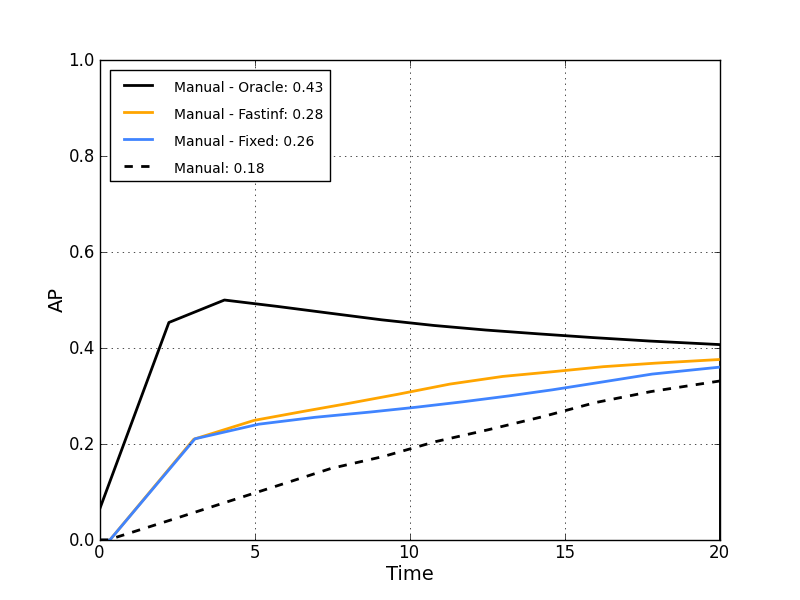
\includegraphics[width=0.78\linewidth]
    {../figures/manual_plots_det_avg.png}} \\
\subfloat[Classification]{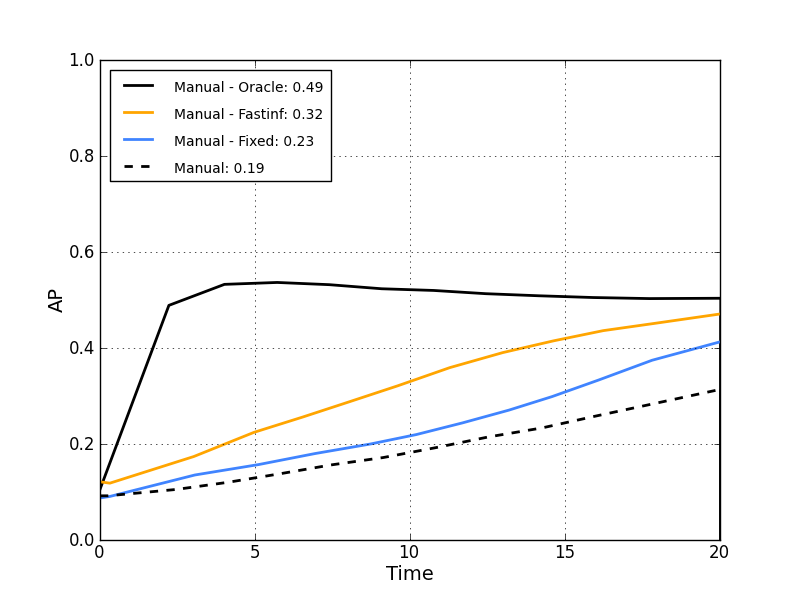
\includegraphics[width=0.78\linewidth]
    {../figures/manual_plots_cls_whole.png}}
  \caption{Heuristic value function.}
  \label{fig:results_manual}
\end{figure}

Figure~\ref{fig:results_manual} also shows the performance of our policy with the heuristic value function and two inference models: the MRF model and a simple fixed-order model that follows the priors.
We can see that due to the dataset bias, the fixed-order policy performs well at first (the person class is disproportionately likely to be in the image), but is overtaken by the proper inference model as execution goes on.

\begin{figure}[h!]
\centering
\subfloat[Detection]{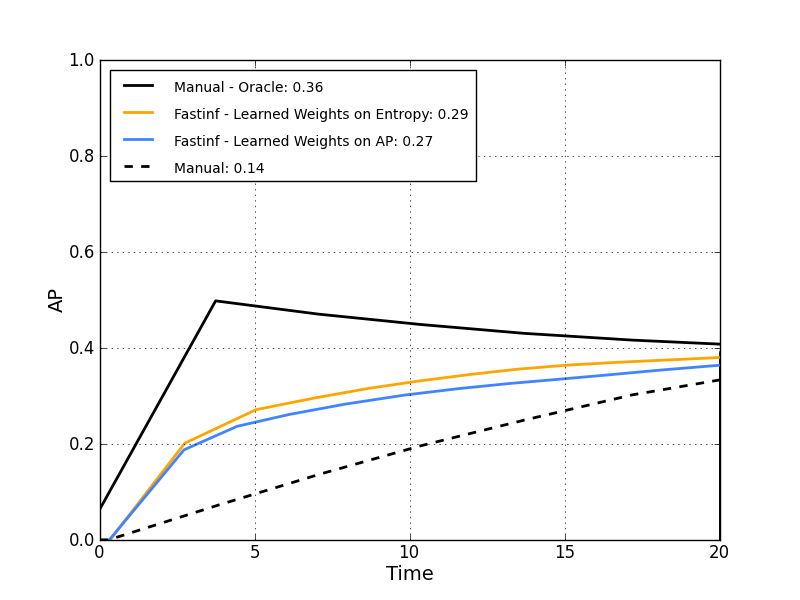
\includegraphics[width=0.78\linewidth]
    {../figures/entropy_plots_det_avg.png}} \\
\subfloat[Classification]{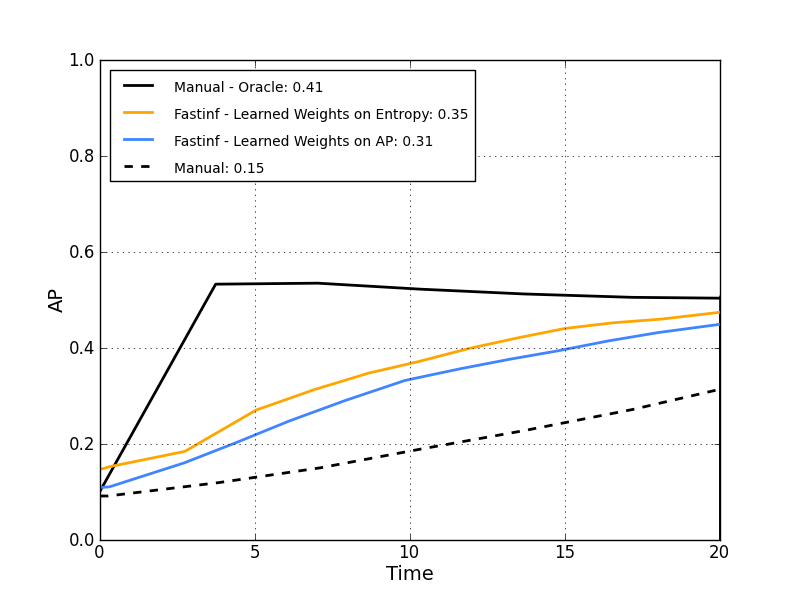
\includegraphics[width=0.78\linewidth]
    {../figures/entropy_plots_cls_whole.png}}
  \caption{Entropy reward function.}
  \label{fig:results_entropy}
\end{figure}

Figure~\ref{fig:results_entropy} shows the performance of the polices with learned weights, comparing our two reward functions.
We found the entropy-based reward to work better than the AP-based reward.

A notable difference between the MRF inference model and the fixed-order model was in the weights learned: while the fixed-order model learned weights onto the bias feature only, the MRF inference model learned weights onto a mix of the entropy and probability features.
\section{Problem Formulation}
Our goal is to output the best detections at some deadline $F$, and to continue having the best detections at every time step after that.
Specifically, we seek to maximize the AP of a detector for all classes in all images of a test dataset.
\note{but see todo note in~\autoref{sec:evaluation}.}

In the limit of infinite time, our program will look everywhere for everything, but given a short deadline, it should first look in the most promising places for the most likely objects.
To take advantage of semantic and spatial context, where it looks at time $t$ should depend on the results gathered by $t-1$.

In each of the $I$ images we consider, we look for $K$ classes of objects, and have detectors $d_k$, with each one having some number $P_k$ of part fittings, cascade stages, or other partial classifiers $c_{kp}$.

We represent an image as a collection of overlapping windows at different scales: a multi-scale pyramid of $N$ locations $\l_i = (x,y,s)$ (the discretization and feautirzation of the image pyramid is discussed in~\autoref{sec:discretization_and_featurization}).
We assume that each location $\ell$ can be the center of at most one bounding box, containing an object belonging to one of $K$ classes.
While this assumption may not hold in cases of occlusion, it does hold for the data we consider and at the levels of discretization we use. \note{is this true?}

\aside{
There are two ways we could think about our task.
The first can be called ``assigning content to locations.''
It fits the sliding-window paradigm.
The second can be called ``assigning locations to content.''
It is inspired by particle filtering and the like~\cite{Gualdi2010}.
We'll mostly talk in the paradigm of the former, but these are two sides of the same coin.
}

We first describe a partially observable Markov decision process representing our problem.
Although we do not commit to using the methodology of solving POMDPs, this section is important, as it describes the specific models we assume, which even a hard-coded solution will use.

We can consider three variants of object detection as a sequential decision problem:
\begin{enumerate}
  \item Looking for everything at a location: Selecting a location $i$, and running a black box program $P$ there that evaluates all detectors as it sees fit.
  \item Looking for something at a location: Selecting a location $i$ and a detector $d_k$. Picking the sequence of partial classifiers for $d$ is then a black box subproblem.
\item Looking for partial evidence of something at a location: Selecting a location $i$ and a partial classifier $c_{kp}$.
\end{enumerate}
We will be working mostly at the level of the third problem in the following sections, although our initial implementations may start out at lower levels.

\subsection{POMDP}
We face a finite-horizon Partially Observed Markov Decision Process (POMDP), which we define as the tuple $(S,A,O,T,\Omega,R,\gamma,F)$, where:
\begin{itemize}
  \item $S$ is a set of discrete states, $A$ is a set of discrete actions, and $O$ is a set of continuous observations.
  \item $T(s,a,s') = P(s_{t+1} = s | a_t = a, s_t = s)$ is the distribution describing the probability of transitioning from state $s$ to state $s'$ upon taking action $a$.
  \item $\Omega(o,s,a) = P(o_{t+1}=o | a_t = a, s_{t+1} = s)$ is the distribution describing the probability of observing $o$ from state $s$ after taking action $a$.
  \item $R(s,a)$ is the reward signal received when executing action $a$ in state $s$.
  \item $F$ is the deadline to first evaluation.
\end{itemize}

The problem is naturally episodic, where an image presents an episode.
Our goal is to learn the optimal policy $\pi$, which is a mapping from histories (trajectories) $h_{1:t}=((a_1,o_1,r_1)...,(a_t,o_t,r_t))$ to actions $a$.

\subsection{State representations}
For all approaches described later, the state $s \in S$ is fully defined by the time $T$, and the class of the bounding box centered at each location.
We augment the $K$ classes with a ``background'' class, which means that there is no object of interest at a location.
Note that each object in the image is assigned to exactly one location; this is in contrast to many detection models employing random fields, such as~\cite{Torralba2004}.
The number of states is exponential in $N$.

An interesting aspect of our task is that we are dealing with a static image, meaning that nothing changes the underlying state.
Therefore, $T(s,a,s') = \delta_{s, s'}$ where $\delta$ is the Kronecker delta function.
In the usual POMDP setting, the physical state is non-stationary, and a repeated action $a$ may lead to different observations $o$.
In our case, it does not make sense to run the same detection action at a location more than once, and so there is a finite number of actions $\mathcal A$ (not just action types) for us to take in an episode.
This means that $F$ can be set to a finite time $F_{max}$, such that all the possible actions can be taken before termination.
This corresponds to an exhaustive search.

Normally in POMDPs, the history $h$ is unbounded (except by the horizon) and quickly becomes intractably large.
For this reason, POMDP policies are either \emph{memoryless}, meaning that the next action depends only on the last observation, or depend on some internal state representation that is a compression of the trajectory.
A common internal representation is the belief state, $P(s|h_{1:t})$, which can compactly represent everything the program needs to know to make Bayesian-optimal decisions.
If the POMDP is known, then we can convert it with this internal representation to an MDP over belief states, and solve it optimally using MDP techniques.
However, this optimal solution approach is hard to scale to large POMDP problems~\cite{Murphy2000,Ng2000}.
We again note that in our problem, the size of $h_{1:t}$ is always bounded by $\mathcal A$.

We model the internal POMDP state as a graphical model, with nodes for the $N$ locations in the image pyramid, and $N$*$K$ possible observations.
A node $y_{i} \in Y$ is an integer $0 \dots K$, according to the class whose bounding box we believe is centered at location $i$ (background is $0$).
A node $z_{ik} \in Z$ is the real-valued output of a detector of class $k$ at location $i$, signifying classifier confidence.
Two nodes $y_i$ and $z_{ik}$ are connected with weight $w_{k}$, which in a sense represents our confidence in the classifier $c_k$ and also allows us to account for multi-class bias.

The connections between two nodes $y_i$ and $y_j$ are defined by the spatial context feature $d_{ij}$ (represented in~\autoref{fig:dij}) and the weights $w_{y_i,y_j}$.
These weights encode valid geometric configurations of object classes $y_i$ and $y_j$.
\begin{figure}[h!]
  \caption{Figure from~\cite{Desai2009}.}
  \centering
    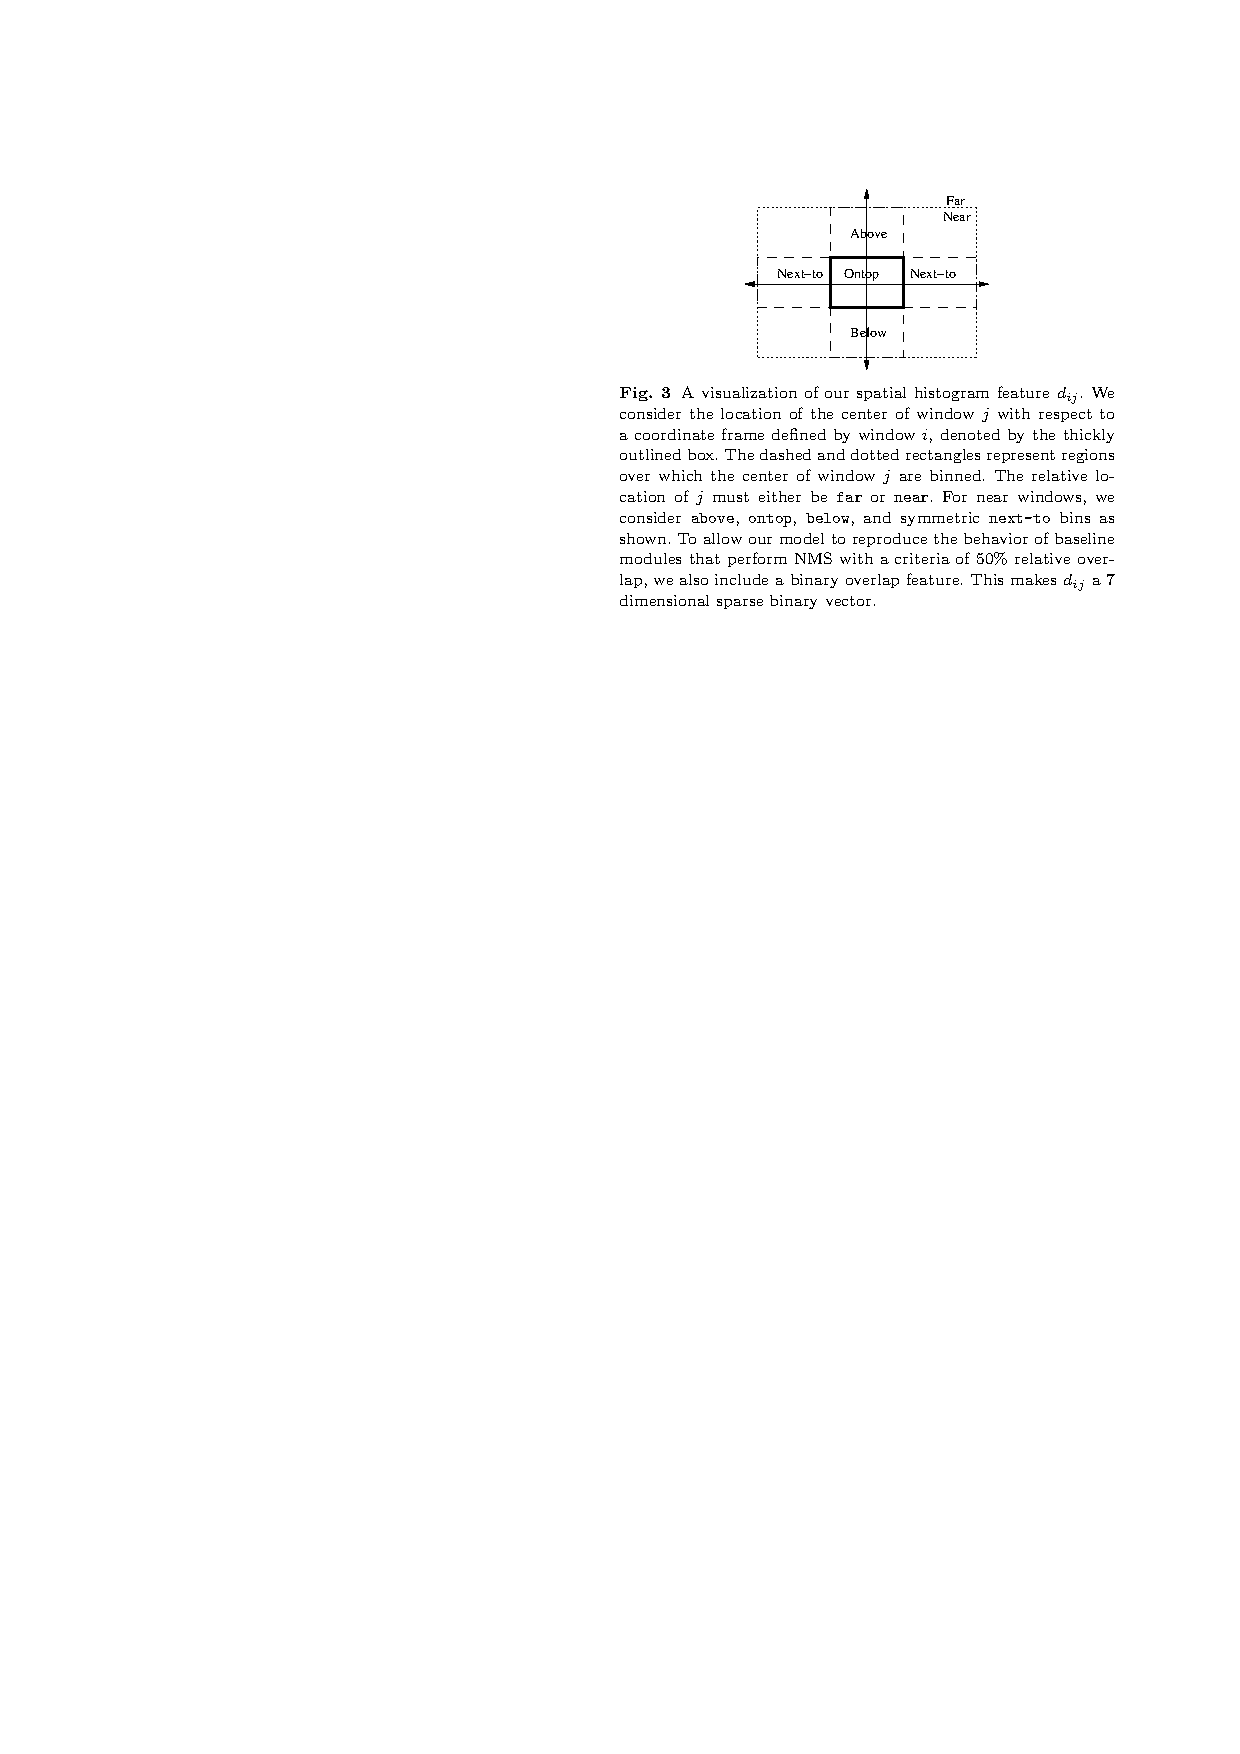
\includegraphics[width=0.7\textwidth]{../figures/dij.pdf}
  \label{fig:dij}
\end{figure}

In this way, we can think of the internal state as a sort of CRF, where $y_i$ are conditioned on the image $X$ through $z_{ik}$.
Crucially, the extra nodes $z_{ik}$ can be unobserved.
This internal state therefore both encodes the full trajectory $h$ (albeit in an orderless way), and provides a model-based probability distribution over $s$.
We note that we do not encode rewards received in the internal representation, and discuss this further in~\autoref{sec:misc}.

This way of modeling the underlying state of the image is similar to the one used in~\cite{Desai2009}.
In fact, we rely on their method of greedy forward search to do inference in the CRF and learn the parameters; inference of the physical state from our belief state is described in~\autoref{sec:rewards}.

\subsection{Actions and Observations} \label{sec:actions}
There are two distinct ways to formulate the action space.

The first defines actions by a choice of location $i$ and detector $c_{k}$, making for $NK$ possibilities.
This action space allows any possible action to be taken at any time, and with the right policy could capture structure of the problem, such as non-maximum suppression and spatial cueing.
The space is considerably large, however, and policies have to be highly complex to be effective.

The second restricts the action space with our domain knowledge of the problem.
For instance, we know there is no point in running the same action twice.
Therefore, we can offer just one action to the agent: ``pick a random unexamined (location,class) pair.''
Of course, the only possible policy then is a random exploration of the space.
To structure the exploration, we can offer action such as ``pick a random class for an unexamined location with the highest entropy of $z_{i}$'' (entropy is discussed in~\autoref{sec:misc}).
We can separate picking the class from picking the location, to for example, obtain a policy of picking an unexplored location of maximum saliency, as determined by some non-state featurization of the image, and picking the class most likely to be in the image, as determined by some other classification output of the image.
Some example policies following this approach are described in~\autoref{sec:example_policies}.

In either case, upon executing an action, the observation $o$ we get back is the confidence of the classifier.
The observation updates the corresponding node $z_{ik}$.
We can propagate this update through the graphical model with an iteration of belief propagation, or alternatively, we can find the MAP assignment to $Y$, given this new information, by running a greedy forward search (details in~\autoref{sec:rewards}).
We can do this at every action, every fixed number of actions, or upon taking a special action.

\subsection{Outputting Detections, Receiving Rewards, and the Deadline} \label{sec:rewards}
$Y$ in our belief state represents the detections, and is conditioned on $Z$.

Recall that we cannot have detections of two different classes at the same location, and that the PASCAL evaluation will penalize all but one detections of the same class at overlapping locations.
For this reason, most detection systems that ``assign content to locations'' like this run a post-processing non-maximum suppression step~\cite{Felzenszwalb2010a}.
In a multi-class setting, it is better to resolve such ambiguities with a principled system to model both inter- and intra-class, and short- and long-range interactions.

Our belief state is modeled after such a system, and we simply run a greedy forward search to maximize the energy of our graphical model to pick our final detections~\cite{Desai2009}.
The energy of the model is given as
\begin{equation}
  S(Y,Z) = \sum_{i,j} w_{y_i,y_j}^T d_{ij} + \sum_{i,k} w_{k} z_{ik}
\end{equation}
In brief, the greedy search starts out with an empty set of detections, and proceeds to pick those $y_i$ that maximize $\Delta S(Y,Z)$.
This method has been shown to be optimal for nearly all images ($\approx98\%$) in the PASCAL set (and compared against Loopy BP and Tree-ReWeighted BP)~\cite{Desai2009}.

The theoretical explanation for this comes from the work on \emph{submodular functions}.
The rough idea is that to maximize functions where adding an element to a large set has less effect than adding an element to a small set, greedy algorithms often have theoretical guarantees of near-optimal performance.
The more pairwise connections are non-positive in the CRF, the more submodular it is.
Since most connections in the image CRF are inhibitory (the CRF mostly performs non-maximum suppression, after all), the theory may apply here.

After every action starting at deadline $F$, $R(s,a)$ is assigned according to the AP of these detections.
The program is not terminated at $F$, but runs to $F_{max}$, which is determined by the time it would take to run every possible detector action once.
Therefore, the reward structure is such that there is a large first reward at $F$, and following rewards at every time step.
It is not clear whether a cost-of-living negative reward should be assigned at each time step; in our toy experiments reported in~\autoref{sec:experiments}, this did not seem to make a difference.
We intend to try both ways on the actual problem.

We express $F$ in units of expected time per action, such that taking action $a$ with time cost $\tau$ advances $T$ by $\tau$.
We determine $\tau$ by averaging the wall clock time of executing $a$; this is done for all $a$ prior to running the POMDP learner.

\subsection{Some Example Policies} \label{sec:example_policies}
We can briefly describe how different detection strategies fit into our framework.
Instead of committing to one strategy, we can define our action space to allow multiple strategies.
We can then find a policy that optimally combines the strategies, perhaps as a function of $T$ and $F$, to maximize the reward under our definitions.

\paragraph{Sliding window, Random, and Saliency-driven}
As described, earlier in the text, our definition of the action space can drive any of these policies.
We first compute a simple, fast self-similarity saliency map for the image (for example, as in~\cite{Alexe2010}).
The internal state is featurized by the location of the current unexamined (picked less than $K$ times) max in the saliency map and the class $k$ of the last action.
The policy could then be to simply sample locations in order of saliency, running all detectors at a location before proceeding to the next.

\paragraph{Class prior or posterior-driven}
On the training set, we compute $K$ canonical object likelihood maps.
We featurize the belief state with the current unexamined (picked less than $1$ time) max of each likelihood map.
Our policy is to run the detector for the class $k$ at the location $i$ with the largest likelihood among these maps.

Of course, with our random field model of the environment, we can compute class posteriors for all locations.
As the policy proceeds, it could start taking belief propagation actions to update the class posteriors and improve the quality of the actions.

\subsection{Unobserved rewards and Augmented MDPs} \label{sec:misc}
Our problem formulation briefly noted an important detail: at test time, the program does not receive rewards.
Therefore, we should not learn a policy that depends on the rewards during execution.
For this reason, there is nothing in our internal state representation that encodes rewards received: the only information is what we currently believe each node $y_i$ to be, and what observations $z_{ik}$ we have made.

We can view the observations $z_i = \{z_{i1}:z_{iK}\}$ as an unnormalized distribution over $y_i$.
Accordingly, we can derive the entropy term $H(z_i)$, which represents our uncertainty in the value of $y_i$.
The idea of adding uncertainty variables to the state space of a decision process is known as Augmented MDPs~\cite{Kwok2004,Roy1999}.
Augmented MDPs have the advantage of increased tractability over corresponding POMDPs, while still retaining the modeling power of allowing uncertainty.
For example, policies can account for the uncertainty in the state through the entropy variables, and direct actions accordingly.
This model has been successfully applied to self-localizing robots~\cite{Roy1999} and to the problem of active sensing in soccer-playing Aibos~\cite{Kwok2004}.

If we model our problem as an Augmented MDP, we will lack one thing: knowledge of the reward function.
Accordingly, we can apply the well-developed array of efficient techniques for model-free reinforcement learning~\cite{Sutton1998}.
Additionally, we can shape the reward function with \emph{a priori} domain knowledge, by, for example, encouraging minimal entropy.

\subsection{Solving the RL problem}
We consider several ways to solve the posed problem.

First, we can attempt to solve the POMDP as a belief-state MDP, computing the state value function for it.
This approach is hard to scale to a problem as large as ours, but efficient methods have been developed for medium-sized problems~\cite{Pineau2006}.

Second, we can solve directly for the $Q(s,a)$ function using reinforcement learning techniques.
For general POMDPs, this seldom works, as the model is likely non-Markovian in $s$.
We consider this approach seriously, because for reasons outlined in ~\autoref{sec:misc}, direct model-free learning could work well for us.
A compromise between this and the first approach was proposed in the $Q_{MDP}$ framework~\cite{Littman1995}, which computes $Q$ as if the environment was Markovian at every future time step past the current one, and so defines $Q(b,a) = \sum_x b(x) Q_{MDP}(x,a)$.
In our toy experiments, we use the technique of Least-squares Policy Iteration~\cite{Lagoudakis2003}, an extension of Least-Squares Temporal Difference learning~\cite{Boyan2002} to model-free learning.
This is an efficient linear method allowing a large number of parameters, and recovering the global maximum of the value function.

Third, we can remember that the ultimate goal is to find the best policy, and search for it directly, forgetting about standard indirect approaches of policy evaluation.
Direct policy search is motivated by indirect approaches' several problems when applied to POMDPs:
\begin{itemize}
  \item $Q$ may be unstable due to non-Markovian $s$; 
  \item function approximation may make it hard for reinforcement learning to converge to a stable policy;
  \item stochastic policies may be better suited than deterministic ones to POMDPs.
\end{itemize}

Direct policy search does not suffer from these problems, but of course has the additional problem of how to parametrize and learn the policy effectively~\cite{Murphy2000,Hauskrecht2000}.
An effective way to represent a policy is as a Finite State Machine~\cite{Hansen1998}, which can lead to efficient search solutions.
The PEGASUS framework samples trajectories most efficiently, allowing fast search through a huge space~\cite{Ng2000}.
A series of reports on the GPOMDP algorithm extend the ideas began in Williams's REINFORCE algorithm~\cite{Williams1992} for policy gradient ascent and review much of the relevant literature~\cite{Baxter1999,Baxter1999a}.
Lastly, the problem of searching for the best policy can be treated at its most basic, as a coordinate ascent problem~\cite{Kohl2004}.

In our opinion, direct policy search is most suitable for general POMDP problems, as it minimizes the assumptions made about the belief state, and at least directly ensures that the policy is improved at each iteration of learning (value function learning does not guarantee this).
However, the special structure of our POMDP, and the possibility of a reasonable representation as an Augmented MDP, leads us to at least try a reinforcement learning approach to our task.
We describe initial experiments to this end in~\autoref{sec:toy_experiments}.
\section{Location Discretization and Feature Computation} \label{sec:discretization_and_featurization}

\paragraph{Location Discretization}
The fewer possible discrete locations $l_i = (x,y,s)$, with $i = 1 \dots N$, we consider, the smaller our state space and therefore the better our reinforcement learning solution for a given amount of computation.
Featurization also takes less time as tolerable coarseness increases.
At the same time, we lose power to match ground truth detections.

There are three factors in the discretization process: the stride of the center point of the window $(x,y)$, and the number of octaves and scales per octave of $s$.

\note{todo: include a figure plotting oracle performance vs. decreasing coarseness of the image pyramid discretization.}

\paragraph{Coarse-to-Fine Evaluation}
The standard scale-invariant approach to detection with a template is to evaluate a template of fixed size over different scales of the image pyramid.
A recent report makes the observation that this approach using high-resolution, part-based models performs worse than scale-variant detection that degrades to using low-resolution, rigid models for detection at small scales of the image~\cite{Park2010}.
They demonstrate state-of-the-art results on a pedestrian detection benchmark.
The authors also note that context is most helpful for small-object detections.

\begin{figure}[h!]
  \caption{Illustration of the idea of using low-res models to approximate the output of high-res models, allowing us to only compute the image pyramid at small scales.}
  \centering
    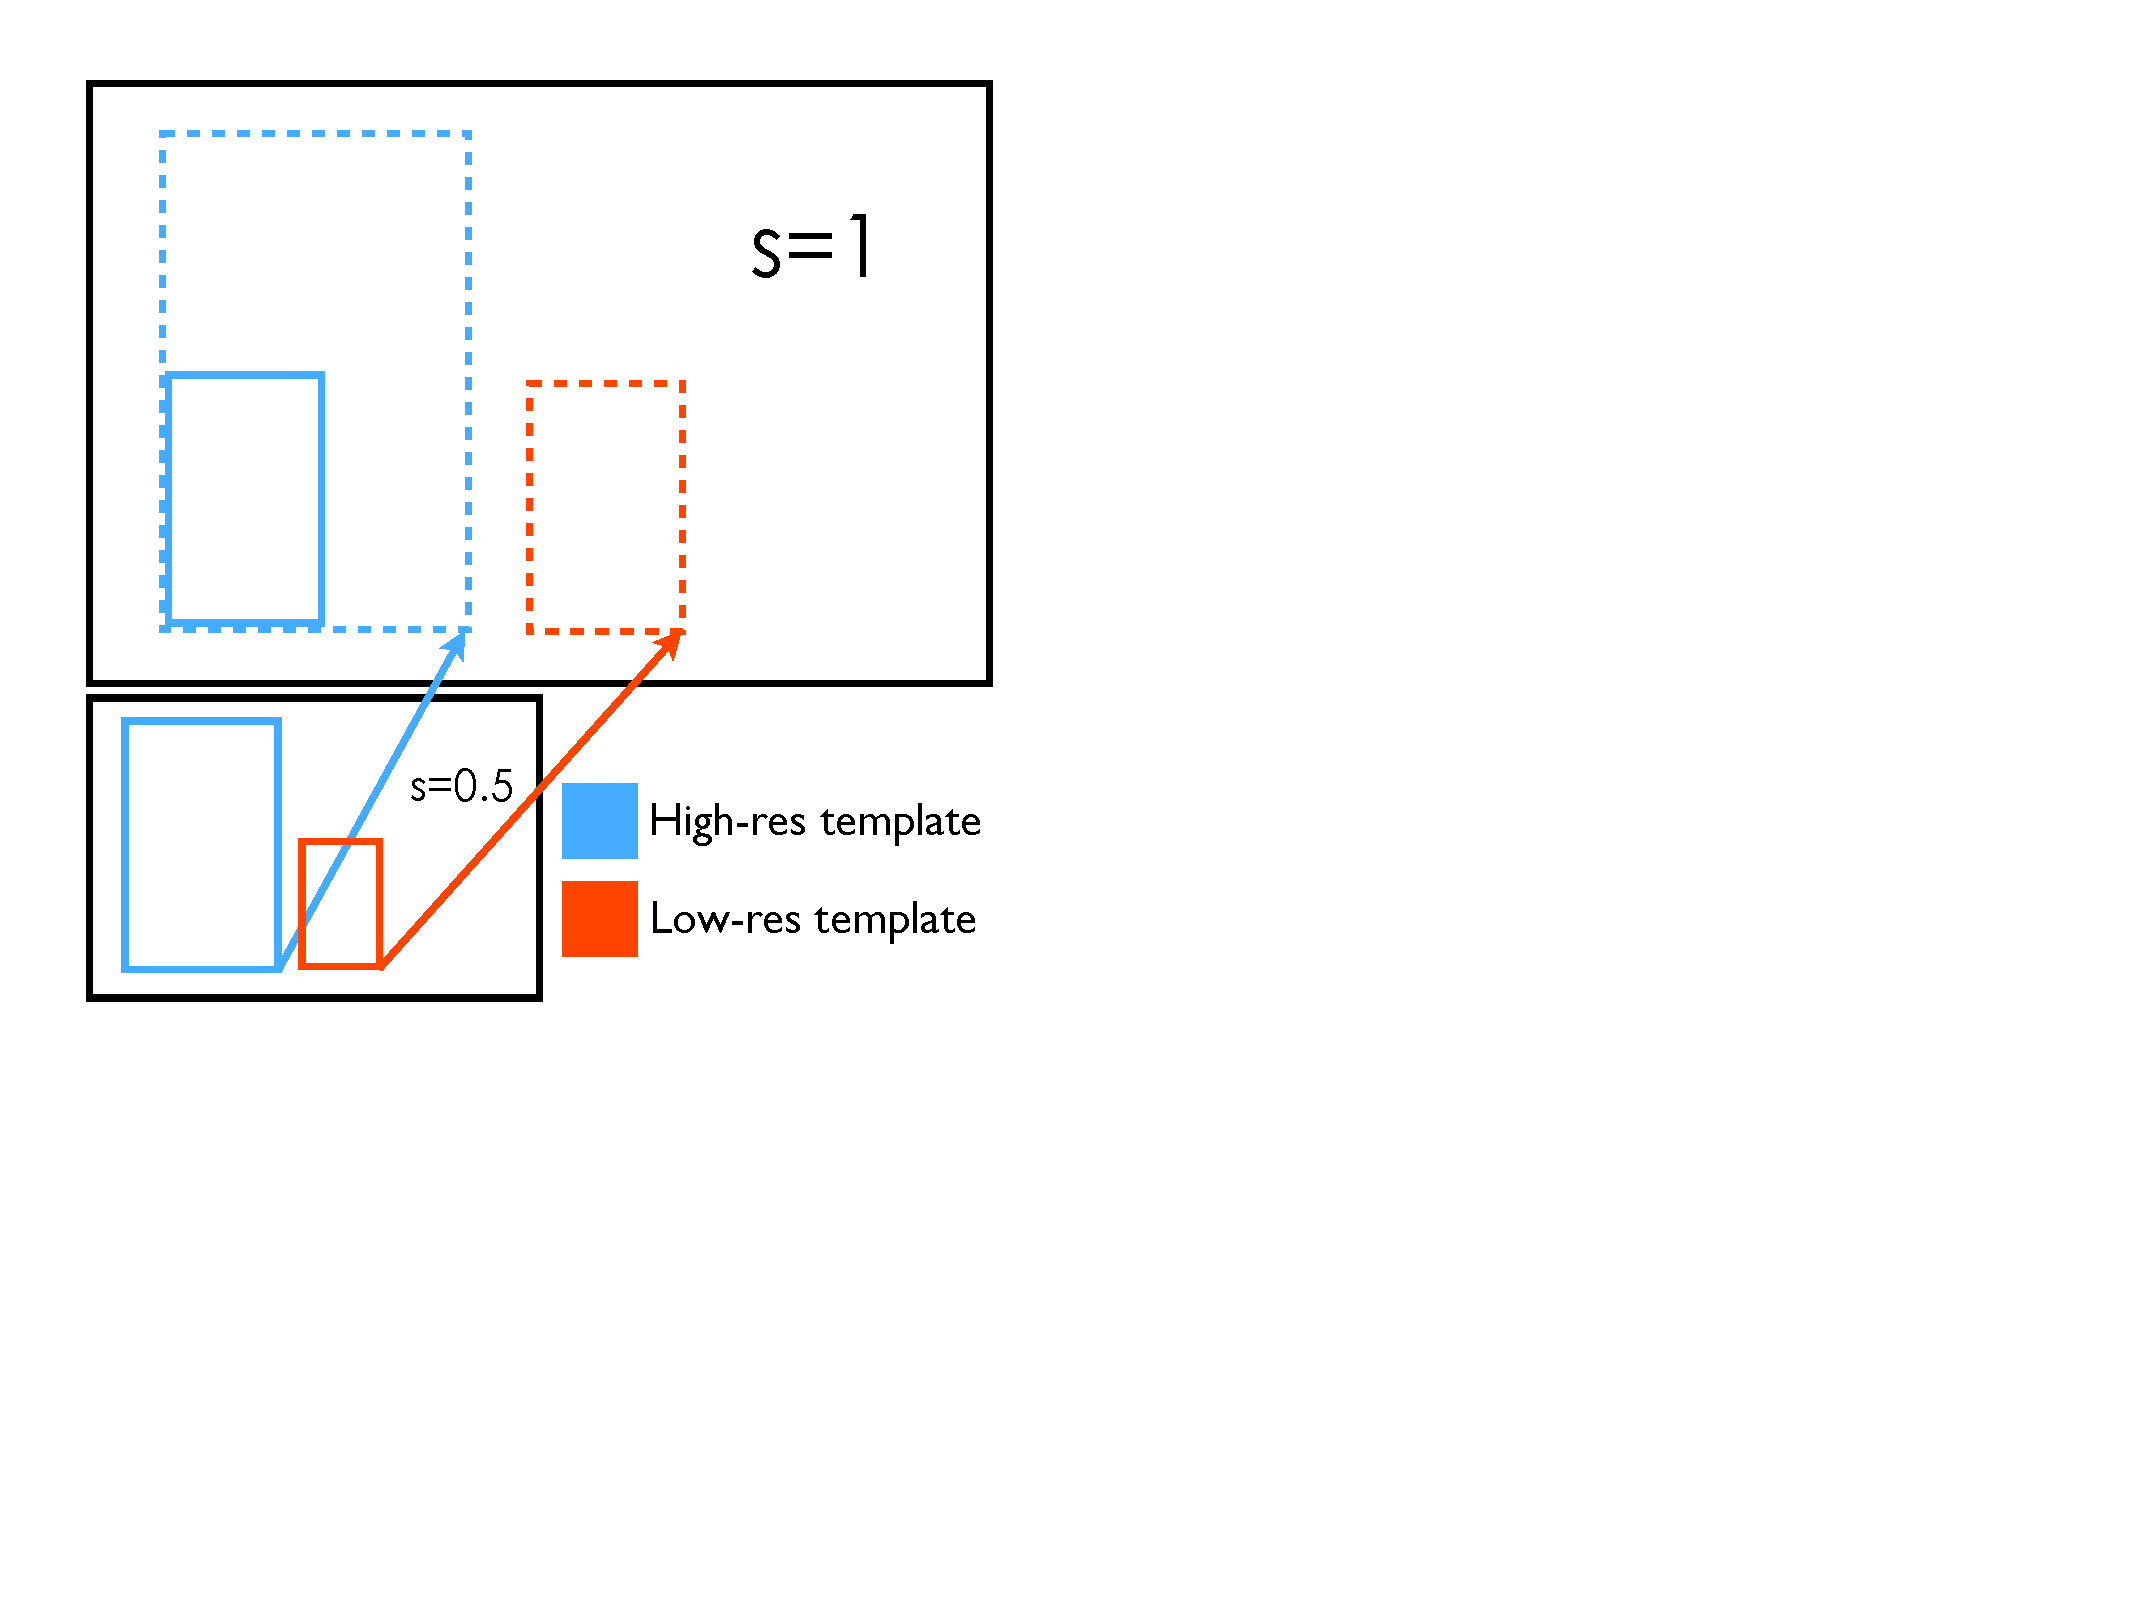
\includegraphics[width=0.7\textwidth]{../figures/multiscale.pdf}
  \label{fig:multiscale}
\end{figure}
We note also that a low-resolution model used at scale $s/2$ provides an approximation to the output of a high-resolution model at scale $s$, as illustrated in~\autoref{fig:multiscale}.
This may allow us to stagger feature computation, first computing just the small-scale part of the pyramid and running low-res models, and then computing the the large-scale part of the pyramid as time allows.

\paragraph{Feature Computation}
\note{todo: how can we include feature computation as part of the action space?}

\note{should look at Piotr Dollar's work on efficient HOG computation~\cite{Dollar2010}.}
\section{Loose Ideas}

\subsection{Local context feature}
We could try augmenting the DPM model with a local context window, for example by learning another HOG template on a window that is slightly larger than the object window.
Has this been done, and why not?
It's also what Allie is thinking of doing for shadow (shadow context around object windows).

\subsection{Fast multi-class approximation of the right class} \label{sec:multiclass_approx}
If we consider a window and have $N$ detectors, how can we efficiently figure out which of the $N$ detectors have the greatest likelihood of giving a high score to this window?

One idea is to use classifier dimensionality reduction.
Let's assume we are using SVM classifiers and classifying vectors of the same dimension.
Do we really need to run all of them in their full dimensions, to have a good guess as to which are going to score high?
Could we not use dimensionality reduction on all the learned classifiers to come up with a very low-dimensional evaluation that would approximate the full-dimensional score?
Then we could only run those classifiers that are past threshold on this low-dimensional approximation.

Another idea is to forget about the specific classifier we are using and just try to partition the feature space into class clusters, roughly.
We can use K-means, for example.
The cluster(s) that a specific window then falls into determine the more complex classifiers that we will evaluate.

\aside{
A similar idea is explored in the paper \cite{Isukapalli2006}.
They use boosting to train a cascade of classifiers to classify all object classes.
Then they learn a policy to partition the output of the detectors into class-specific clusters.
The policy is a decision tree.
The leafs of the decision trees specify the expected class of that window, and they use that to run a class-specific classifier cascade.
}
\section{Results}

We want to show two things: 1) given the same amount of time as our baseline systems, we perform at least as well as them; 2) in the AP vs. time evaluation, we do better than all baselines.

\begin{description}
  \item[Cascaded DPM Baseline~\cite{Felzenszwalb2010b}] We should do as well as it does in the same time ($\approx$0.5 sec), and better than it for shorter times than that.
  \item[Coarse-to-fine Baseline~\cite{Pedersoli2011}] Same thing.
\end{description}

We should think of ways to make the comparison fair.

Should we run the multi-class NMS~\cite{Desai2009} over the detections of the baselines?
Since our approach relies on it, it seems that we should; on the other hand, it's part of the special sauce of our approach.

To make sliding window detectors run faster, we can modify the stride or scale quantization of their sliding window.
So, if we want to output detections in 0.1 seconds, we can modify the Cascaded DPM code, for example, to cover the image in that long.

\aside{
We should also evaluate on some kind of video object detection, to showcase the attentional priors.
Could be an easy CVPR'12 submission.
}

\bibliographystyle{ieeetr}
\small
\bibliography{sergeyk-bibtex}
\end{document}
